\documentclass{beamer}
\usetheme{Madrid}
\usepackage[T1]{fontenc}
\usepackage[utf8]{inputenc}
\usepackage{lmodern}
\usepackage{graphicx}
\title{Atividade 2: Auditoria Forense e Plano de Resgate Tecnico}
\subtitle{Projeto: langfuse/langfuse}
\author{Equipe: Dean Vinícius Palmeira de Meneses; Hilton Hunaldo Costa Silva Brito}
\date{2026-05-31}

\begin{document}

\begin{frame}
  \titlepage
\end{frame}

\begin{frame}{Principais riscos identificados}
  \begin{itemize}
    \item Acoplamento de providers de IA em multiplas camadas (alto impacto para troca).
    \item TODOs em filas criticas (ingestao e webhooks) indicando riscos latentes.
    \item Orquestracao centralizada em um unico fluxo (SRP fragil).
  \end{itemize}
\end{frame}

\begin{frame}{Eixo A: Gestao (MPS.BR GPR)}
  \begin{itemize}
    \item Evidencia de investigacao tecnica e mudanca de escopo em issue \#13933.
    \item Riscos ocultos em TODOs de filas e LLM.
    \item Cadencia de commits consistente, mas revisao humana nem sempre explicita.
  \end{itemize}
  \vspace{0.6em}
    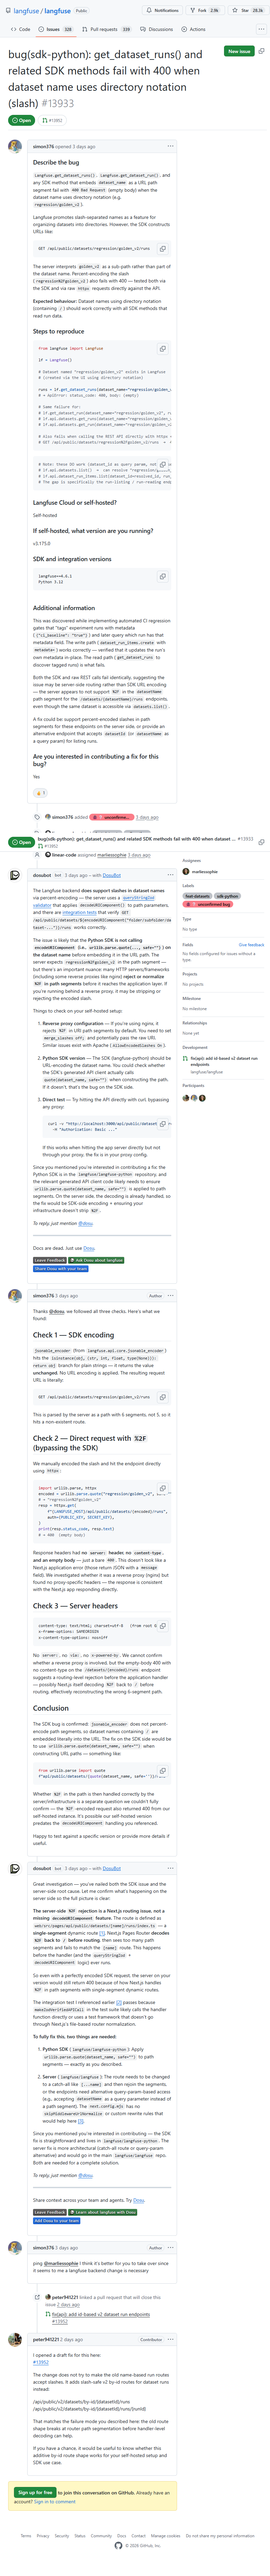
\includegraphics[width=0.49\linewidth]{prints/a1-issue-body.png}\hfill
    
\includegraphics[width=0.49\linewidth]{prints/a2-otelIngestionQueue-main.png}\\[0.35em]
    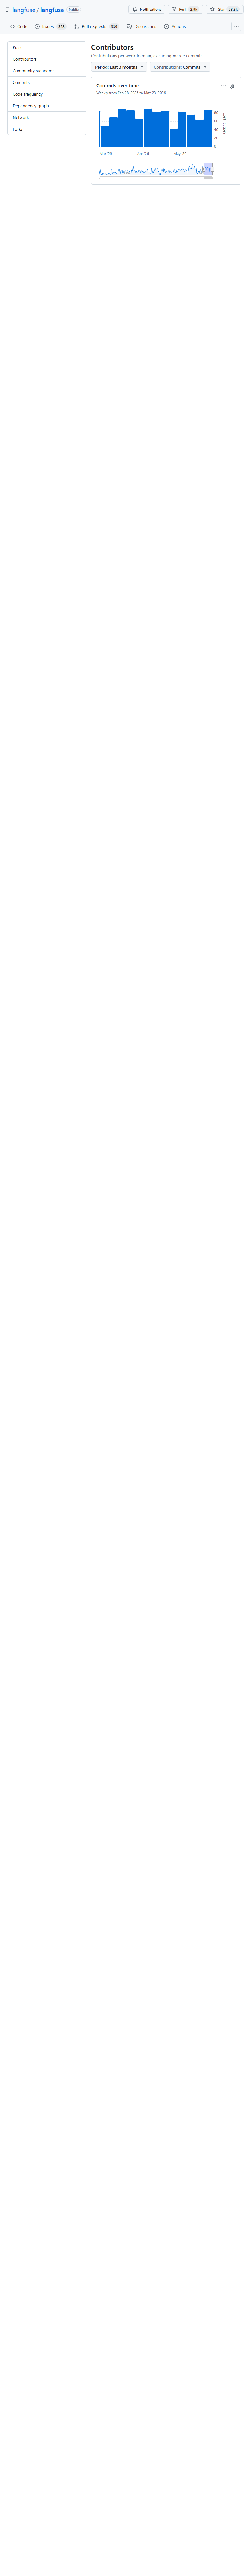
\includegraphics[width=0.49\linewidth]{prints/a3-contributors.png}\hfill
    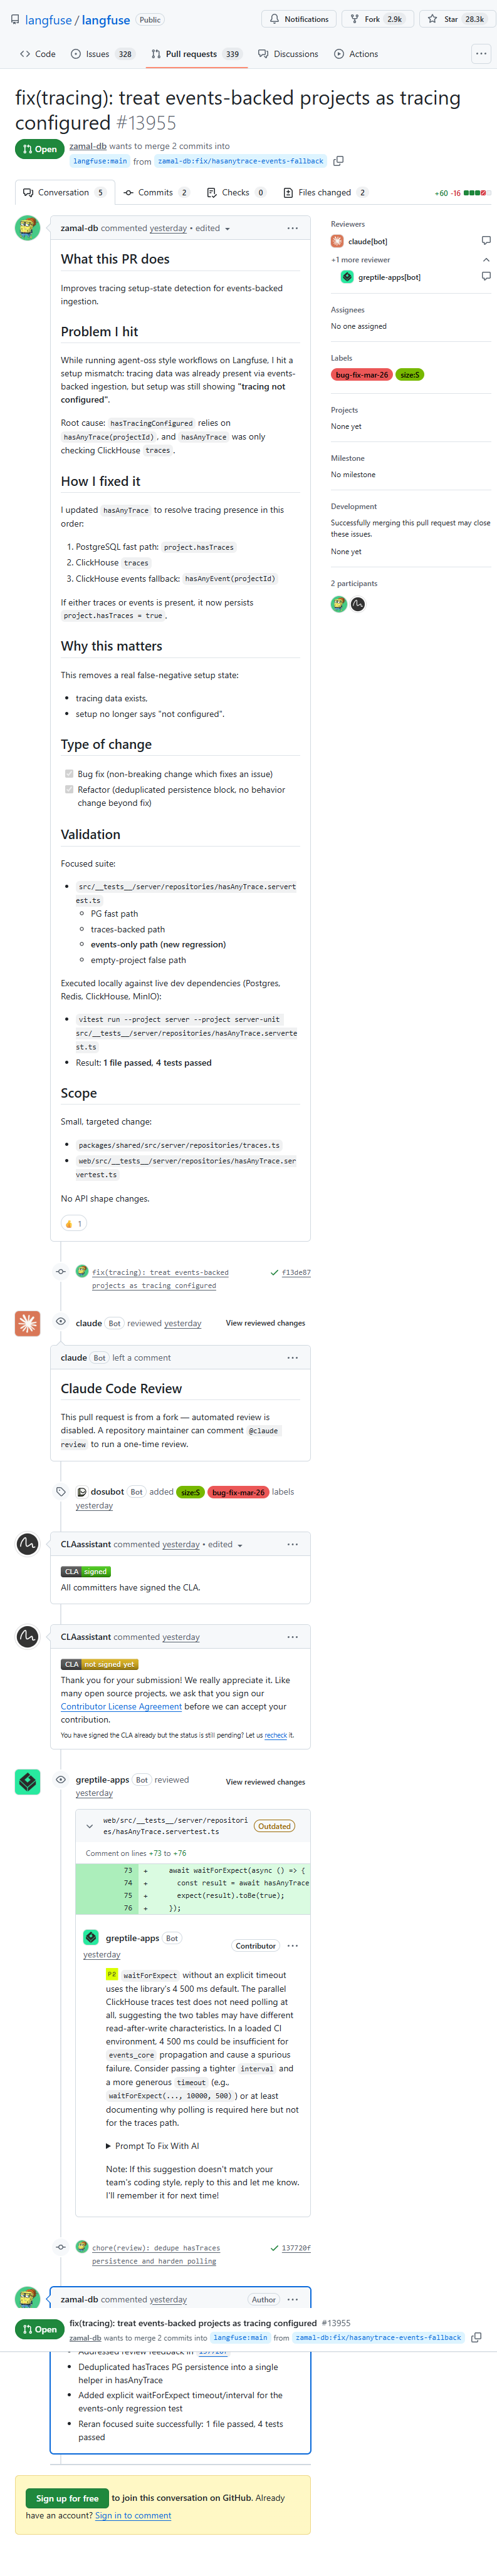
\includegraphics[width=0.49\linewidth]{prints/a3-review-comment.png}
\end{frame}

\begin{frame}{Eixo B: Anatomia do Codigo (SOLID/DRY)}
  \begin{itemize}
    \item Teste da troca mostra logica espalhada por shared/server/UI.
    \item ``God object'': fetchLLMCompletion concentra responsabilidades.
    \item DRY violado em duplicacao de tree building.
  \end{itemize}
  \vspace{0.6em}
    
\includegraphics[width=0.49\linewidth]{prints/b1-types-adapters.png}\hfill
    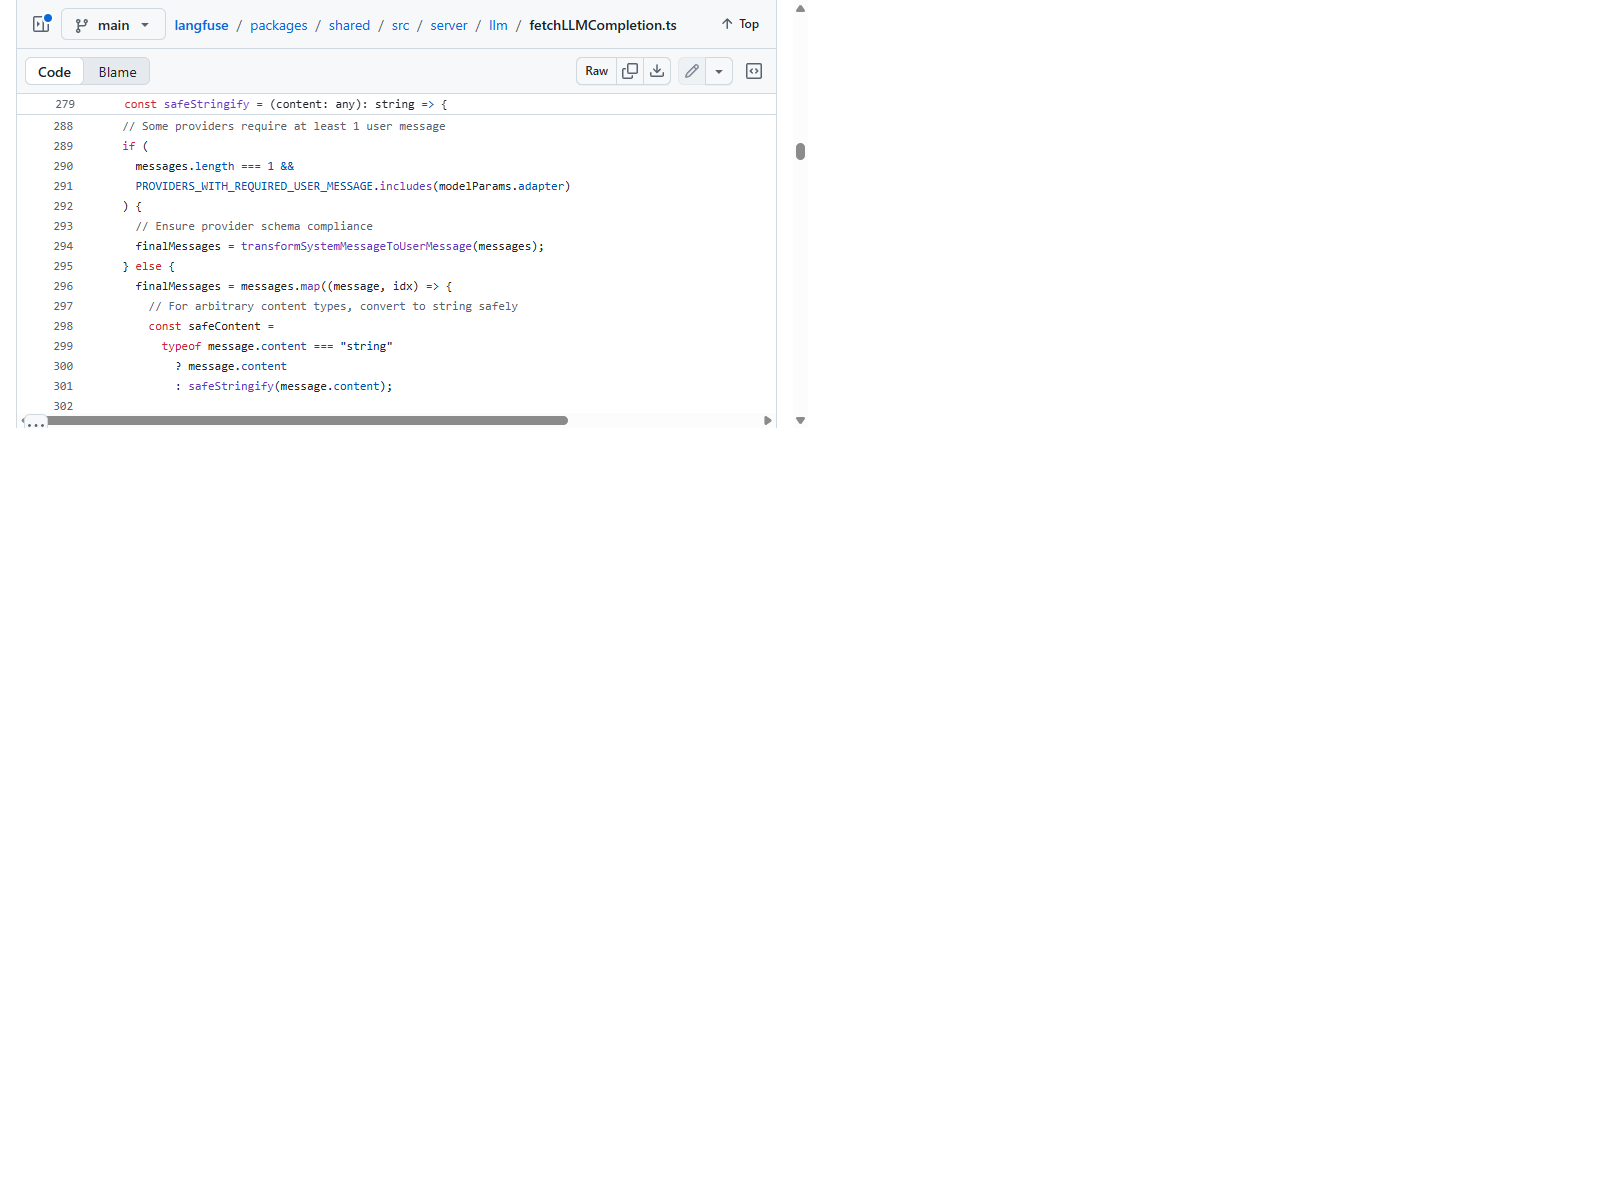
\includegraphics[width=0.49\linewidth]{prints/b1-fetchLLMCompletion.png}\\[0.35em]
    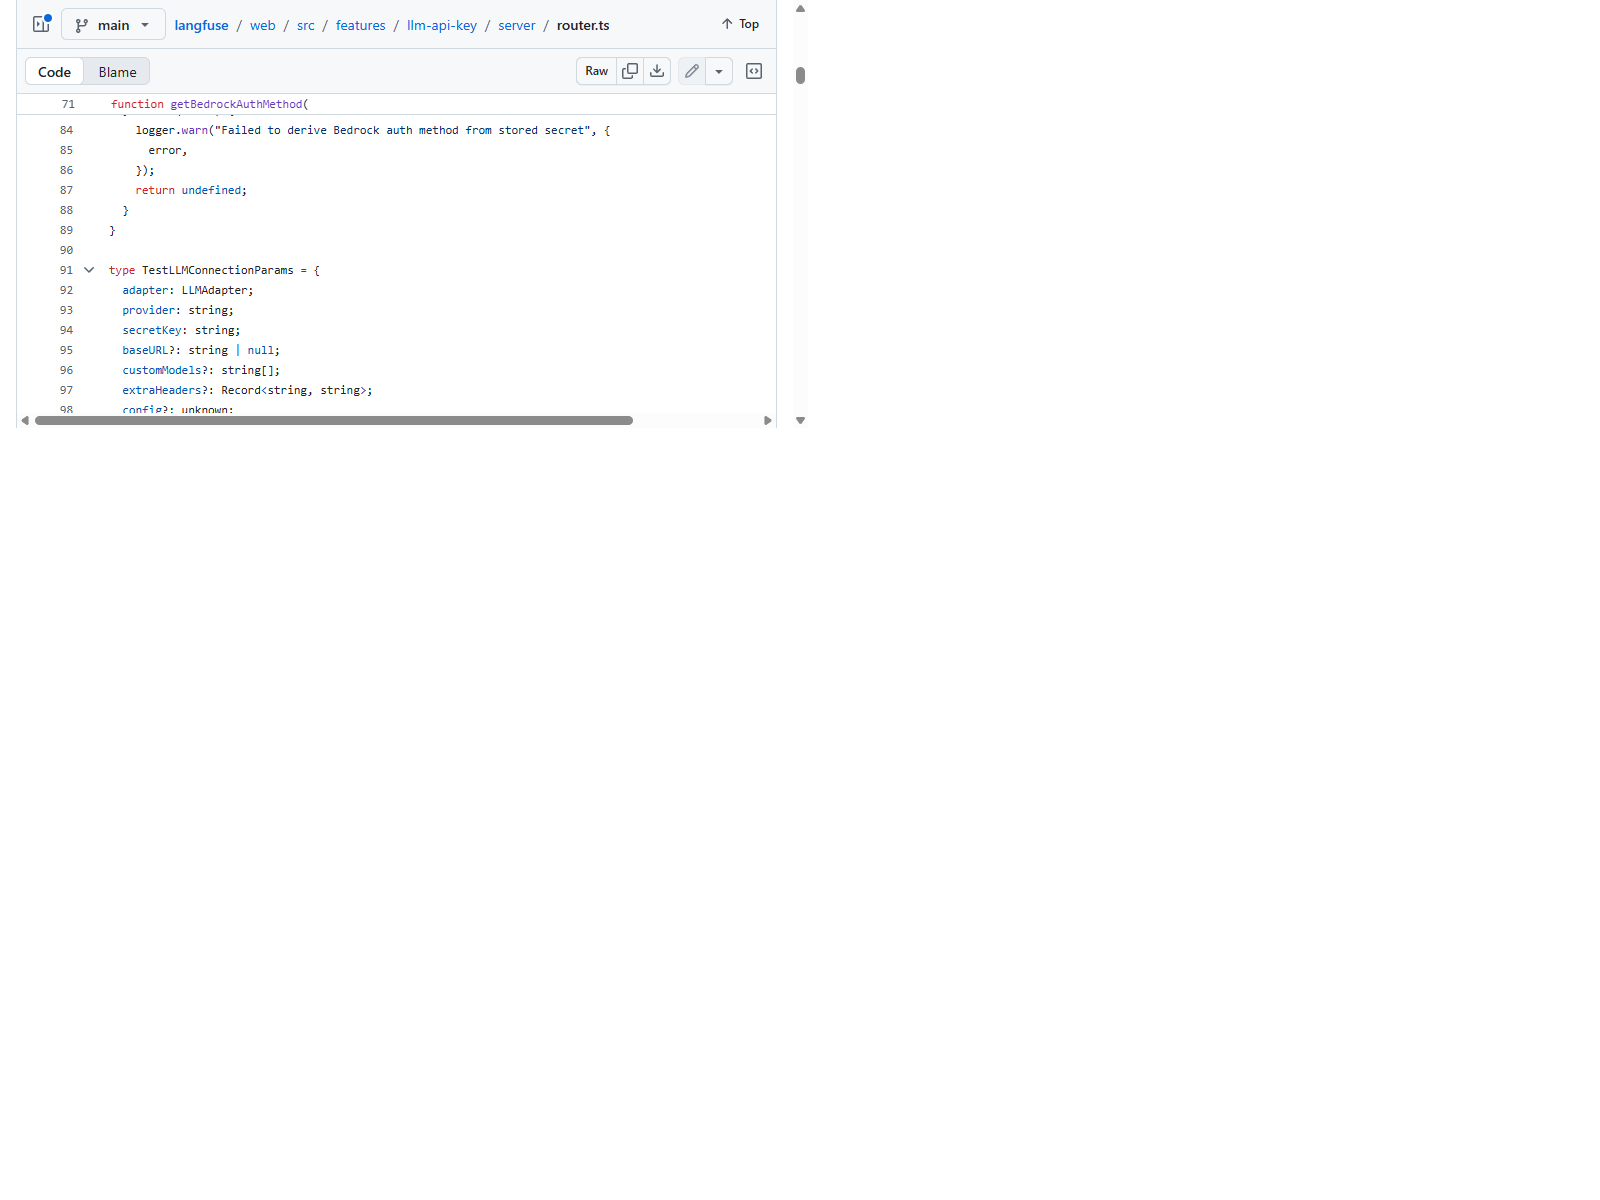
\includegraphics[width=0.49\linewidth]{prints/b1-router.png}\hfill
    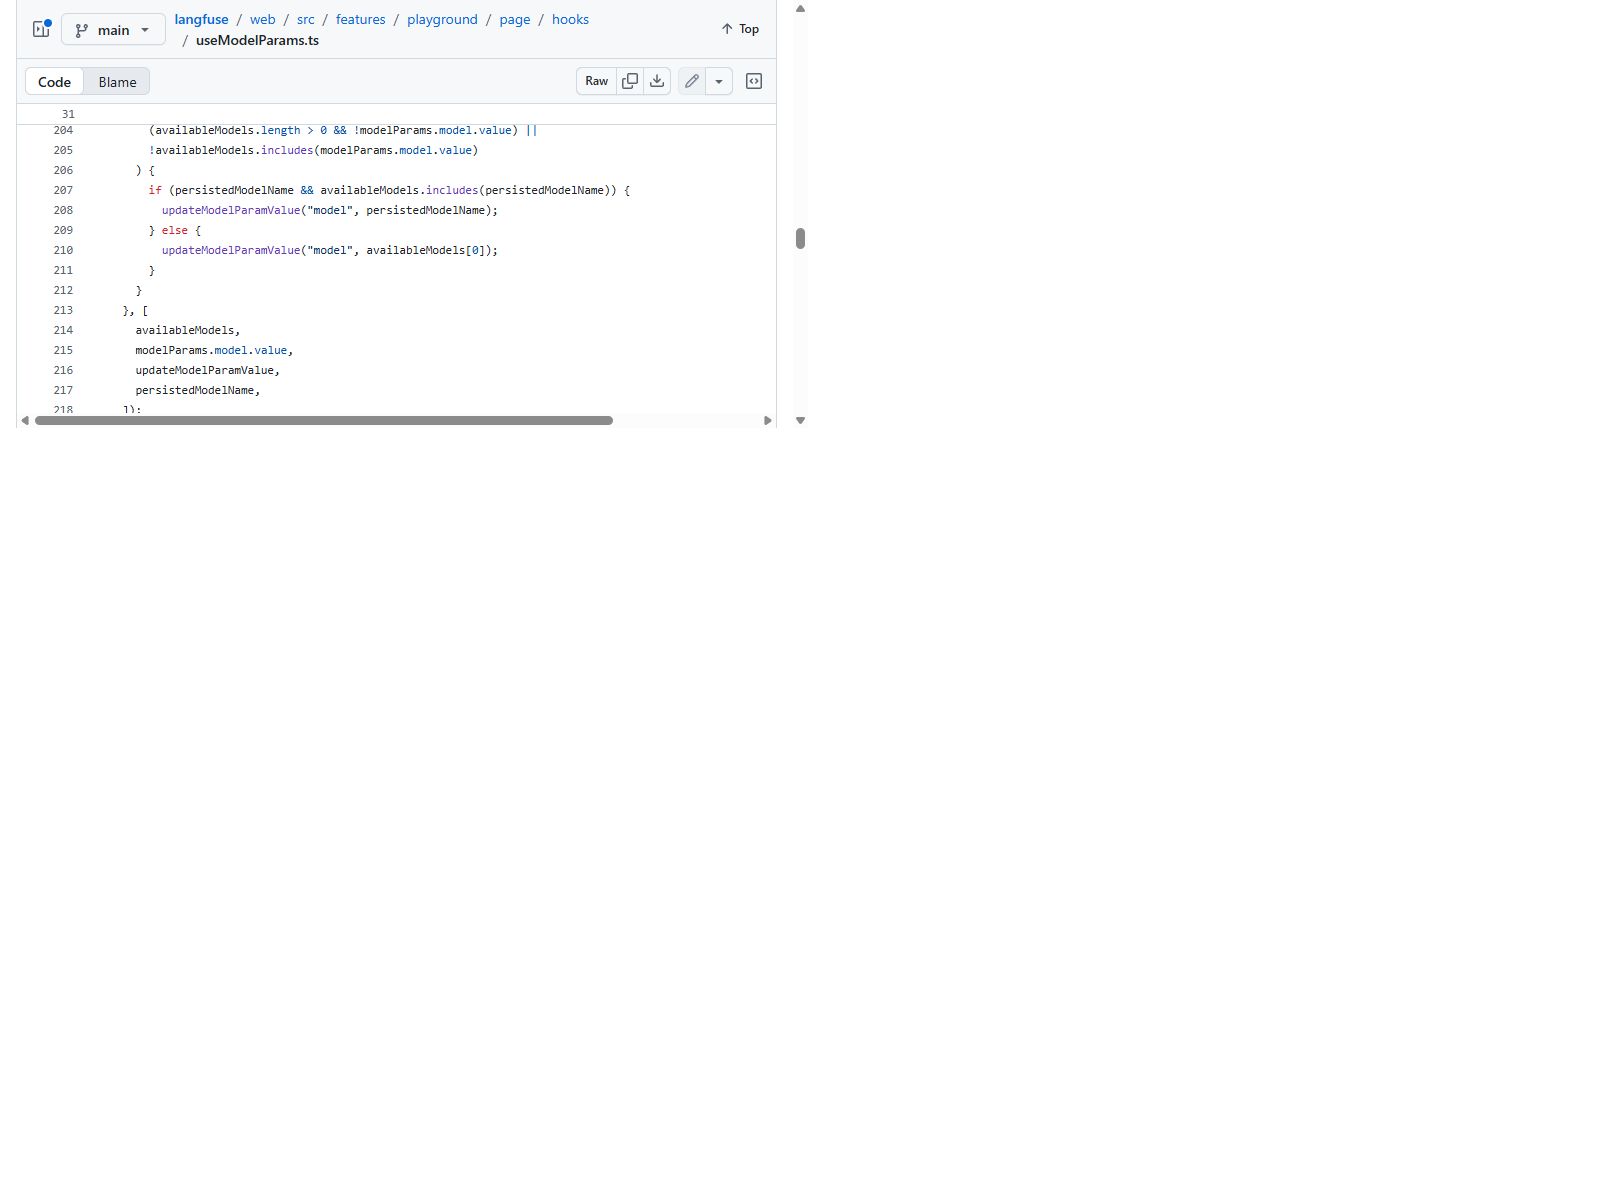
\includegraphics[width=0.49\linewidth]{prints/b1-useModelParams.png}\\[0.35em]
    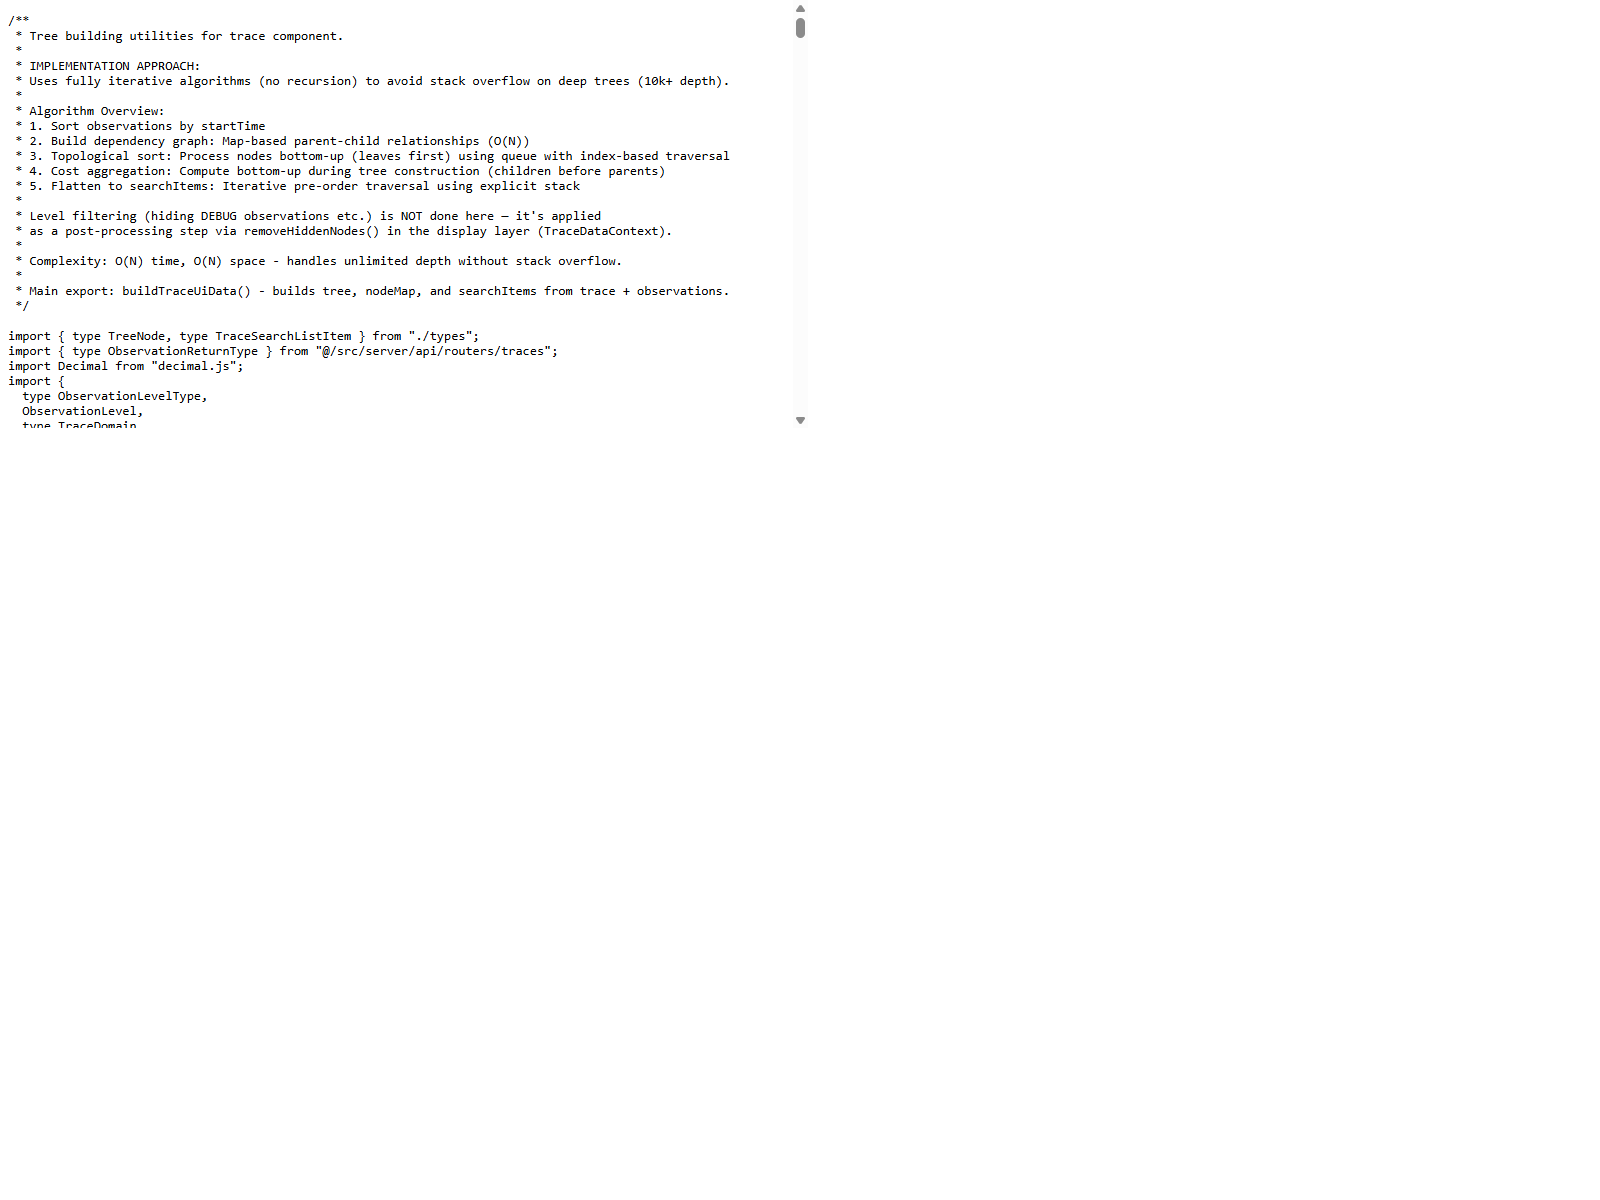
\includegraphics[width=0.49\linewidth]{prints/b3-tree-building.png}\hfill
    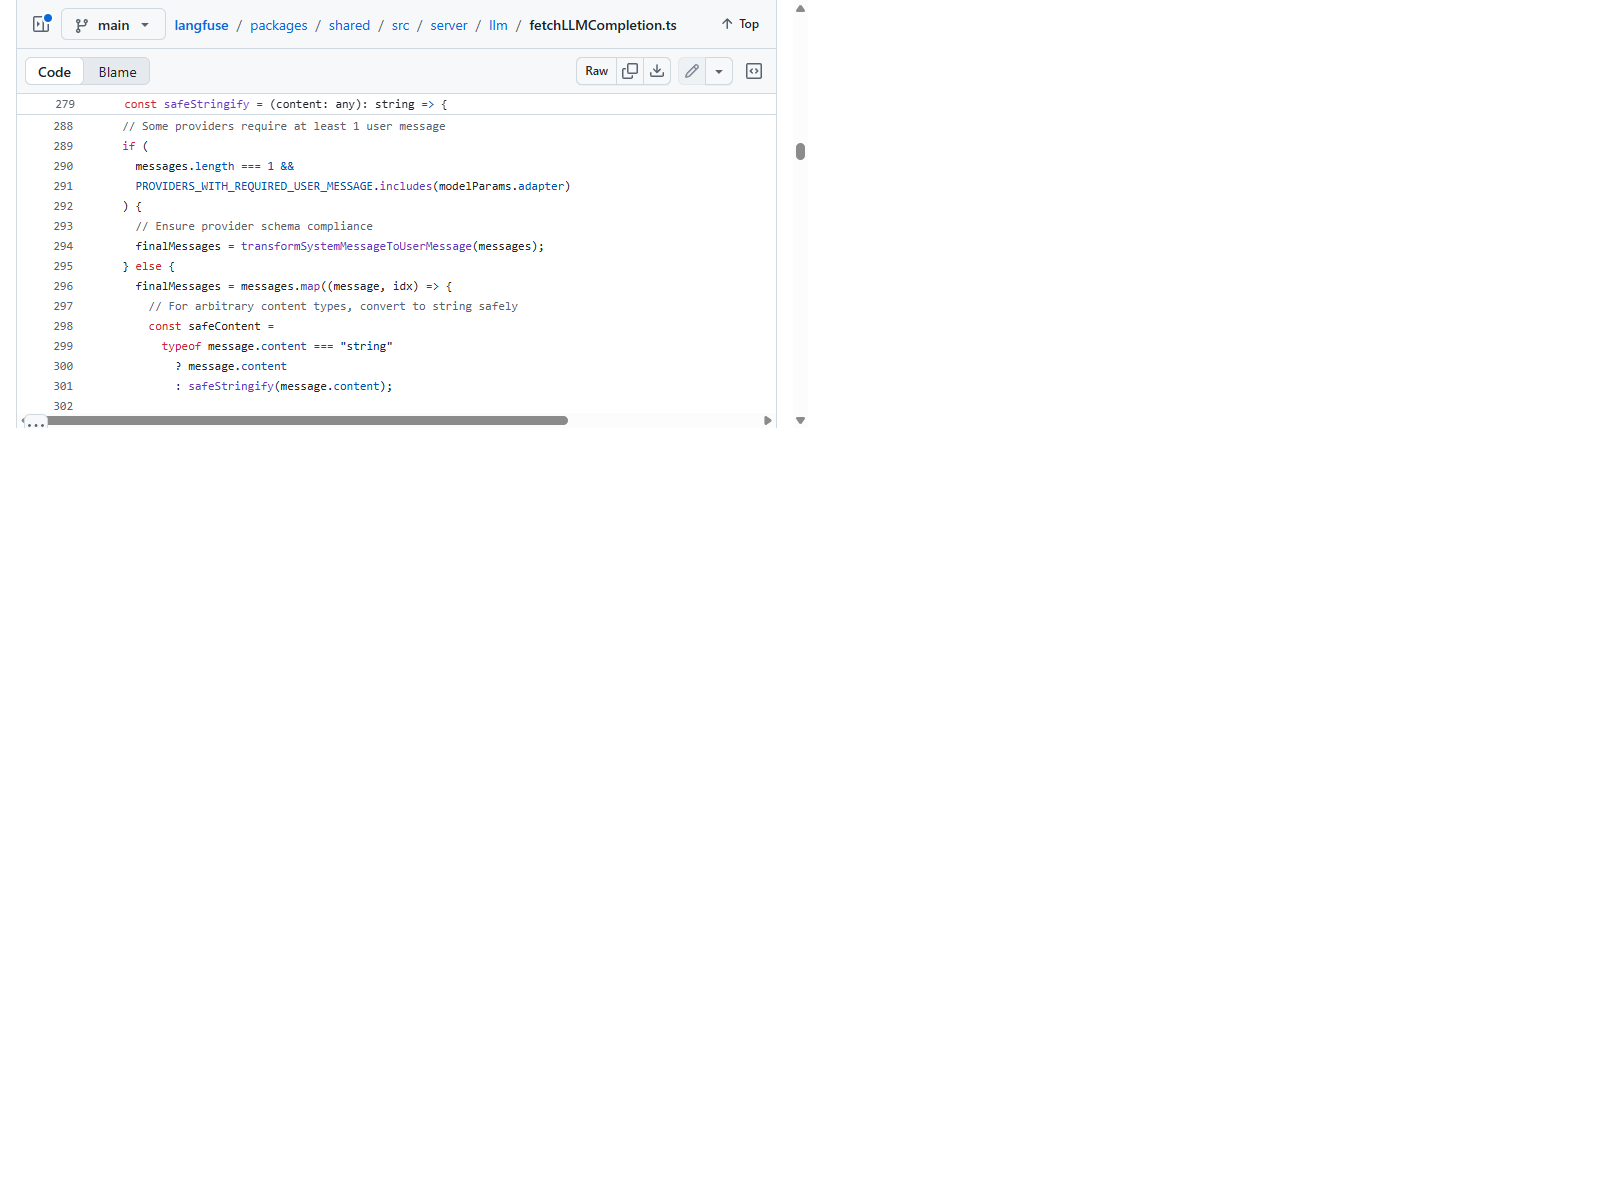
\includegraphics[width=0.49\linewidth]{prints/b2-god-object-fetchLLMCompletion.png}
\end{frame}

\begin{frame}{Eixo C: Padroes GoF}
  \begin{itemize}
    \item Criacionais: Singleton (PrismaClient, SlackService).
    \item Estruturais: Adapter para normalizacao de frameworks.
    \item Comportamentais: ausencia de Strategy/Chain centralizado.
  \end{itemize}
  \vspace{0.6em}
    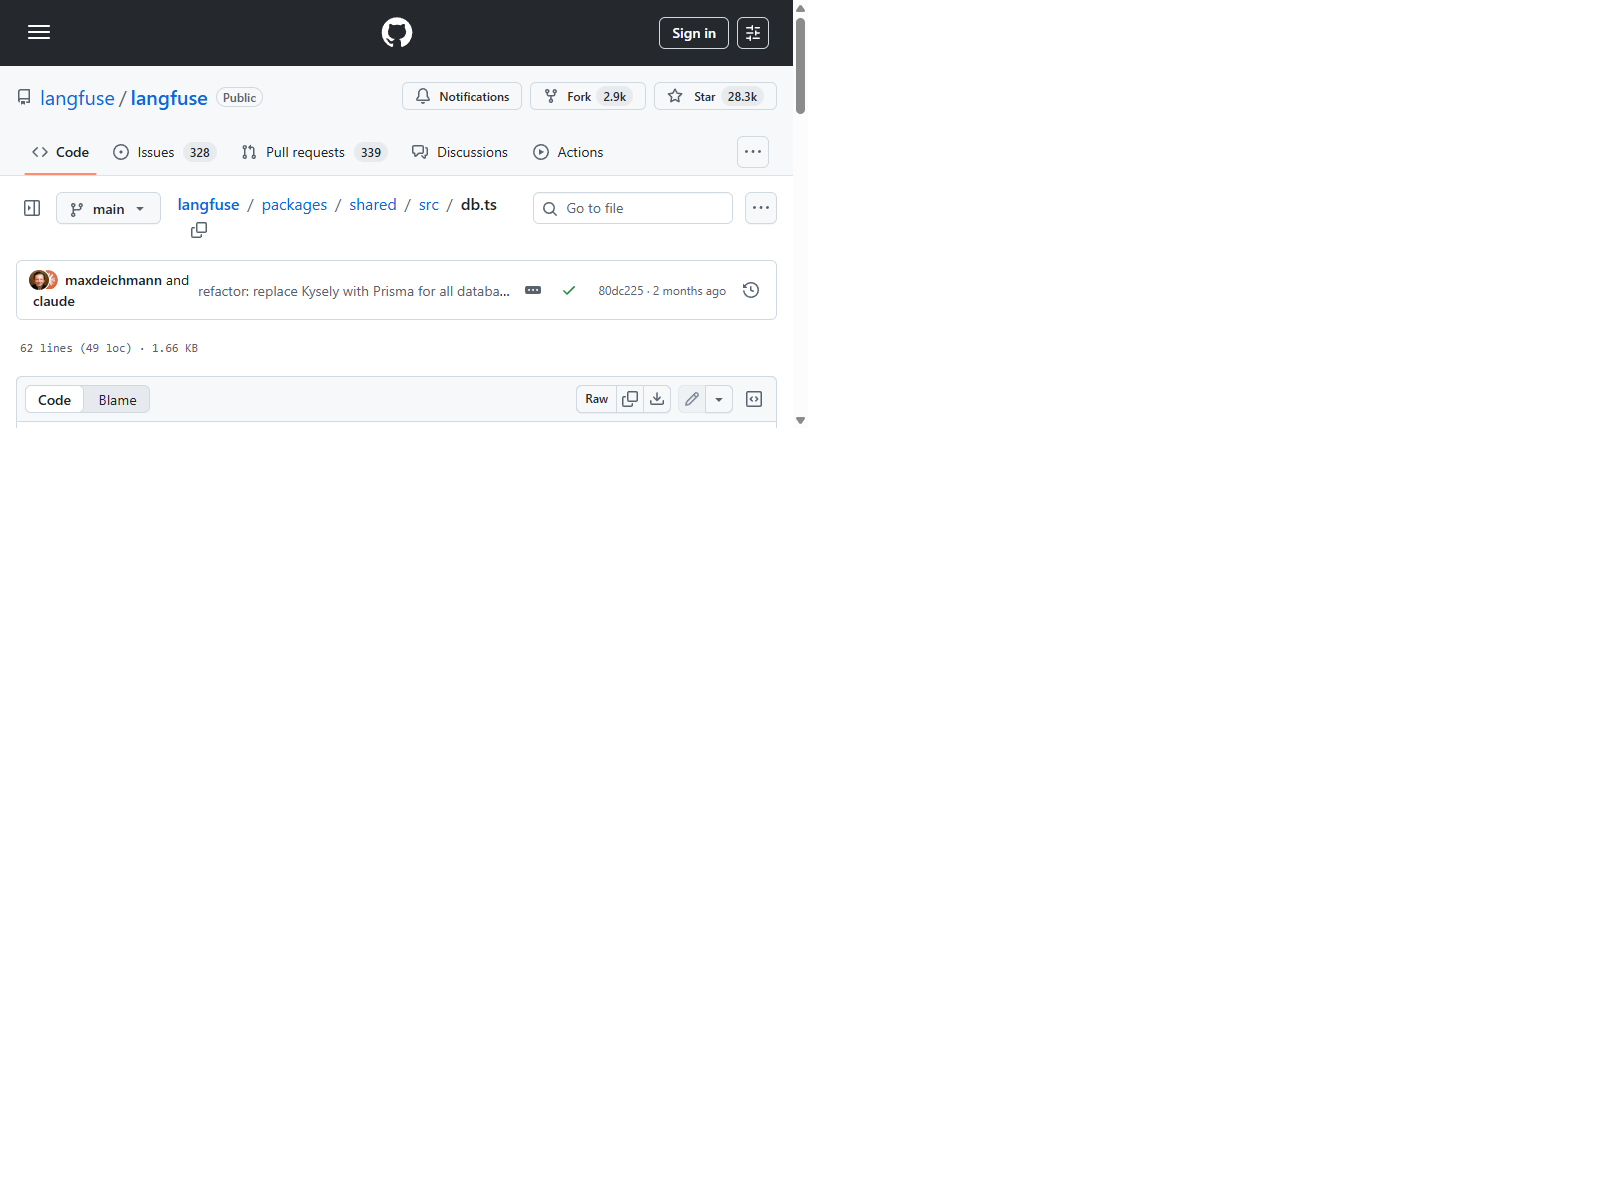
\includegraphics[width=0.49\linewidth]{prints/c1-db-singleton.png}\hfill
    
\includegraphics[width=0.49\linewidth]{prints/c1-slack-singleton.png}\\[0.35em]
    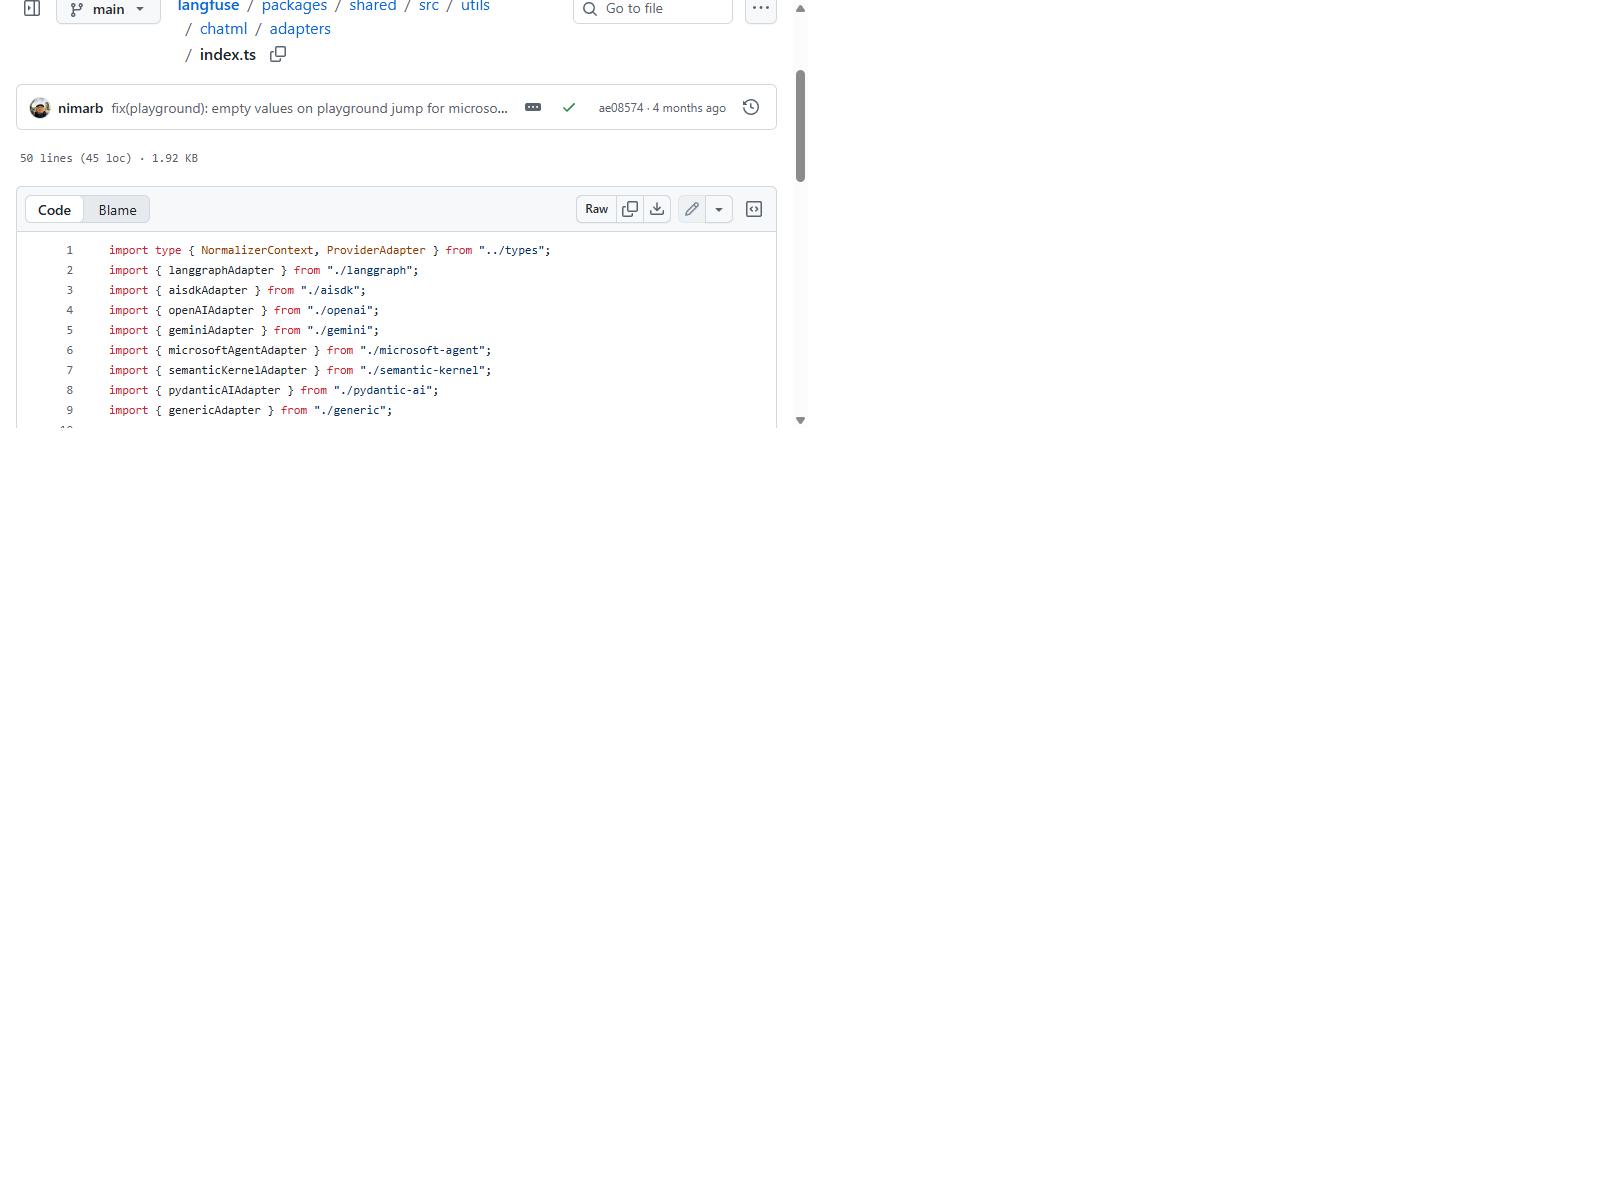
\includegraphics[width=0.49\linewidth]{prints/c2-adapter-registry.png}\hfill
    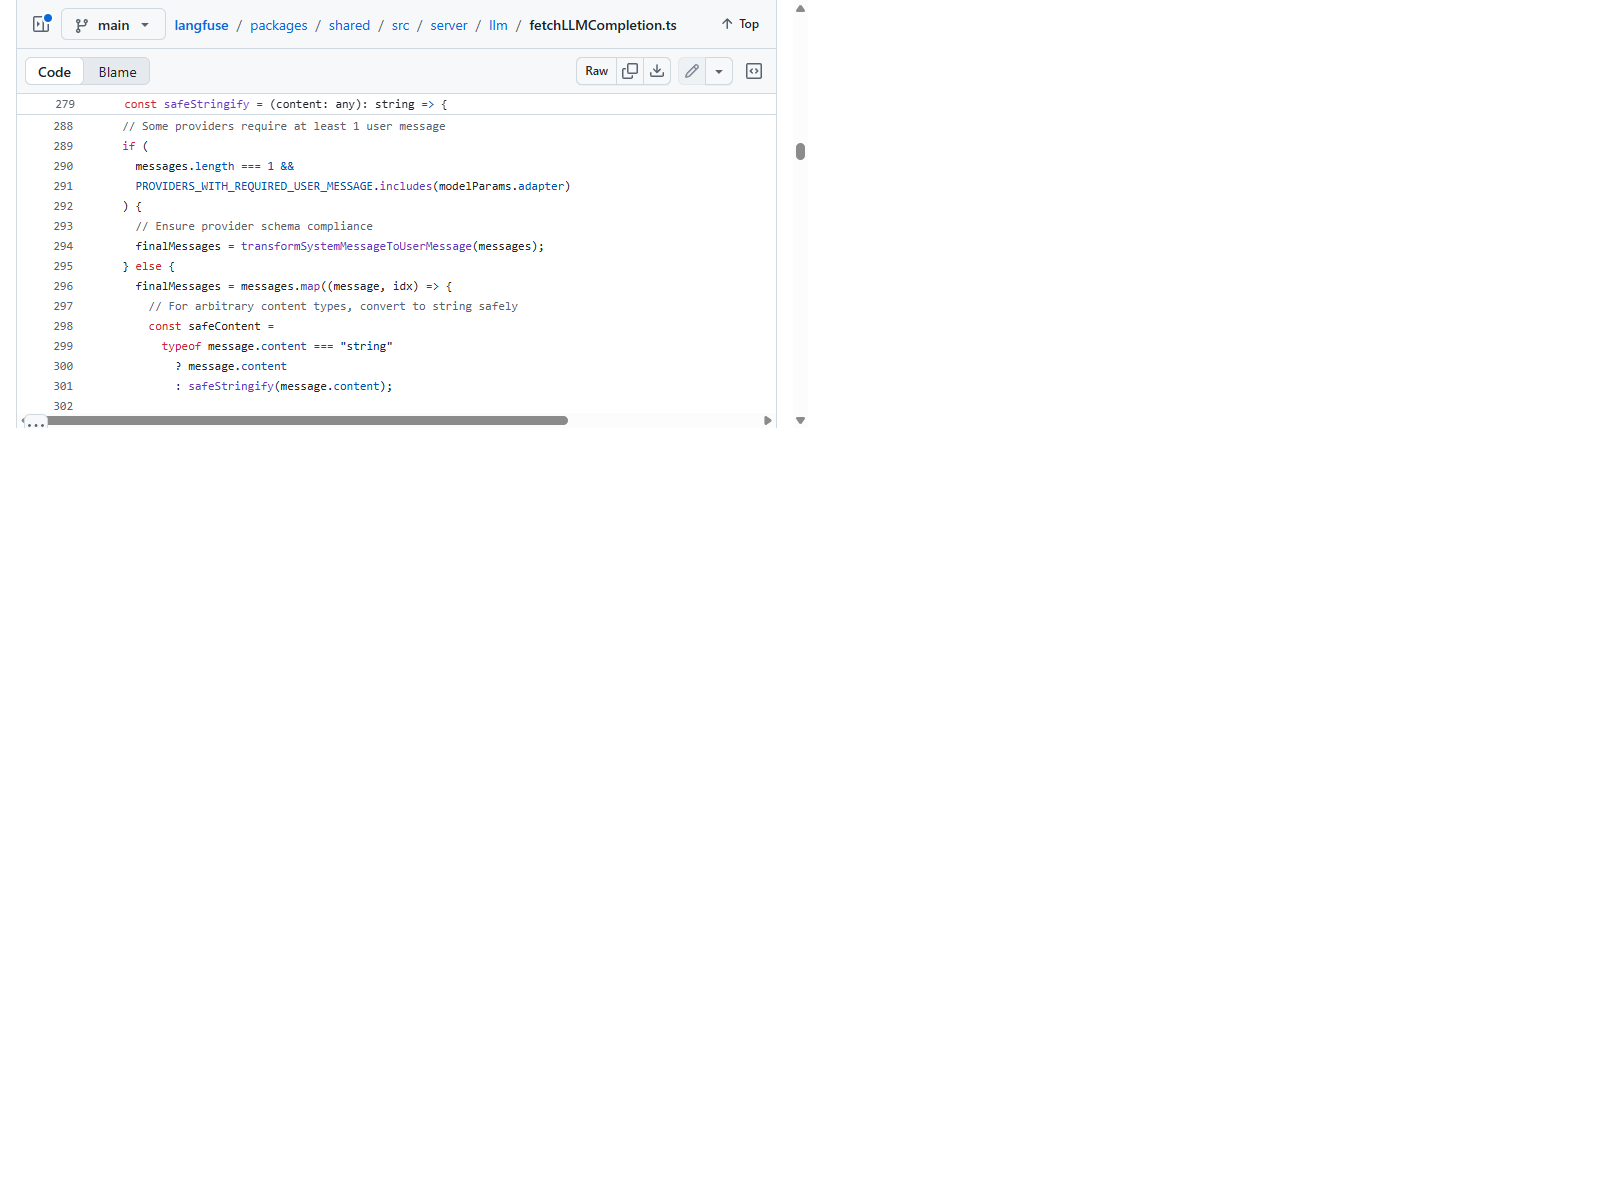
\includegraphics[width=0.49\linewidth]{prints/b2-god-object-fetchLLMCompletion.png}
\end{frame}

\begin{frame}{Plano de Resgate}
  \begin{itemize}
    \item Refatoracao conceitual: Strategy + Registry por provider.
    \item Roadmap MPS.BR G:
      \begin{itemize}
        \item Planejamento com baseline e milestones.
        \item Rastreabilidade requisito -> issue -> PR -> teste.
        \item Registro de riscos + politica de code review.
      \end{itemize}
  \end{itemize}
\end{frame}

\begin{frame}[fragile]{Refatoracao conceitual (exemplo)}
\begin{verbatim}
interface LLMProviderStrategy { ... }
registry.get(adapter).buildClient(...)
\end{verbatim}
  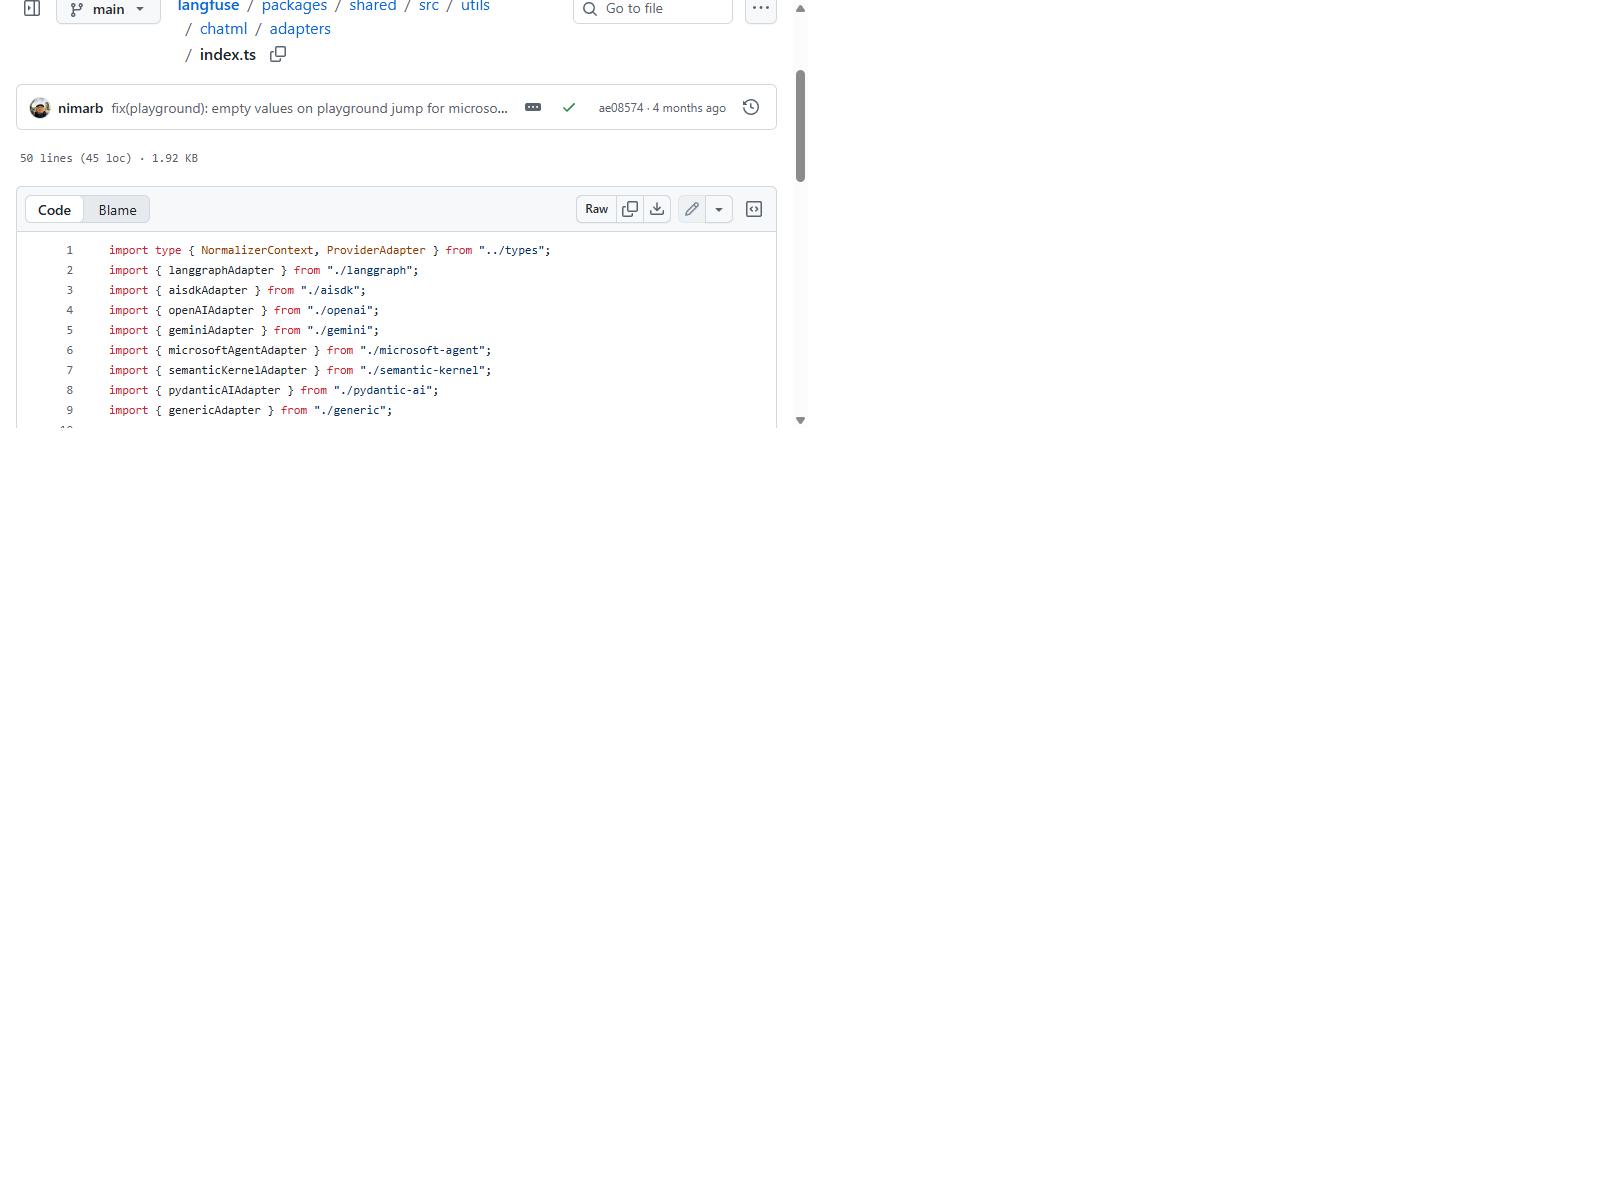
\includegraphics[width=0.82\linewidth]{prints/c2-adapter-registry.png}
\end{frame}

\begin{frame}{Encerramento}
  \begin{itemize}
    \item Resultado: riscos priorizados e plano de resgate alinhado ao MPS.BR.
    \item Proximo passo: executar as 3 acoes iniciais e medir reducao de risco.
  \end{itemize}
\end{frame}

\end{document}
